\clearpage
%%=========================================
% Den litt rare section-formuleringen er for å en kortere header-tittel siden den er for lang ellers.
% \sectionmark{} inne i {section title as seen in paper ...} er for å få riktig header der en section begynner på en oddetallsside.
%
%   \section[section title as seen in TOC]{section title as seen in paper%
%       \sectionmark{section title as seen in header}}\sectionmark{section title as seen in header}
%
%\section[Surface Analysis of Substrate A with Surface Pre-Growth Preparation]{Surface Analysis of Substrate A with Surface Pre-Growth Preparation%
%    \sectionmark{Surface Analysis of Pre-Growth Substrate A}}\sectionmark{Surface Analysis of Pre-Growth Substrate A}\label{sec:subAb}
    
\section{Surface Analysis of Substrate A after Etching}
As substrate A was already polished by the vendor, and the surface pre-growth preparation consisted of simply a \ce{Br}:methanol etch. The dark field images taken of substrate A after etching show that the etch has left more particles on the surface than before, see Fig.~\ref{fig:subAa_om_df} and Fig.~\ref{fig:subAb_om_df}. The density of particles and features larger than \SI{0.5}{\micro\metre} has increased from \SI{\sim 4e2}{\centi\metre^{-2}} to \SI{\sim 1e3}{\centi\metre^{-2}} near the centre of the substrate. \todo{Bare etsing får til flere partikler? Hvor kommer de fra? Løsnet fra kantene og løst seg i esevæsken for så å falle ned. settle on the substrate surface. }

\begin{figure}[htbp]
    \centering
    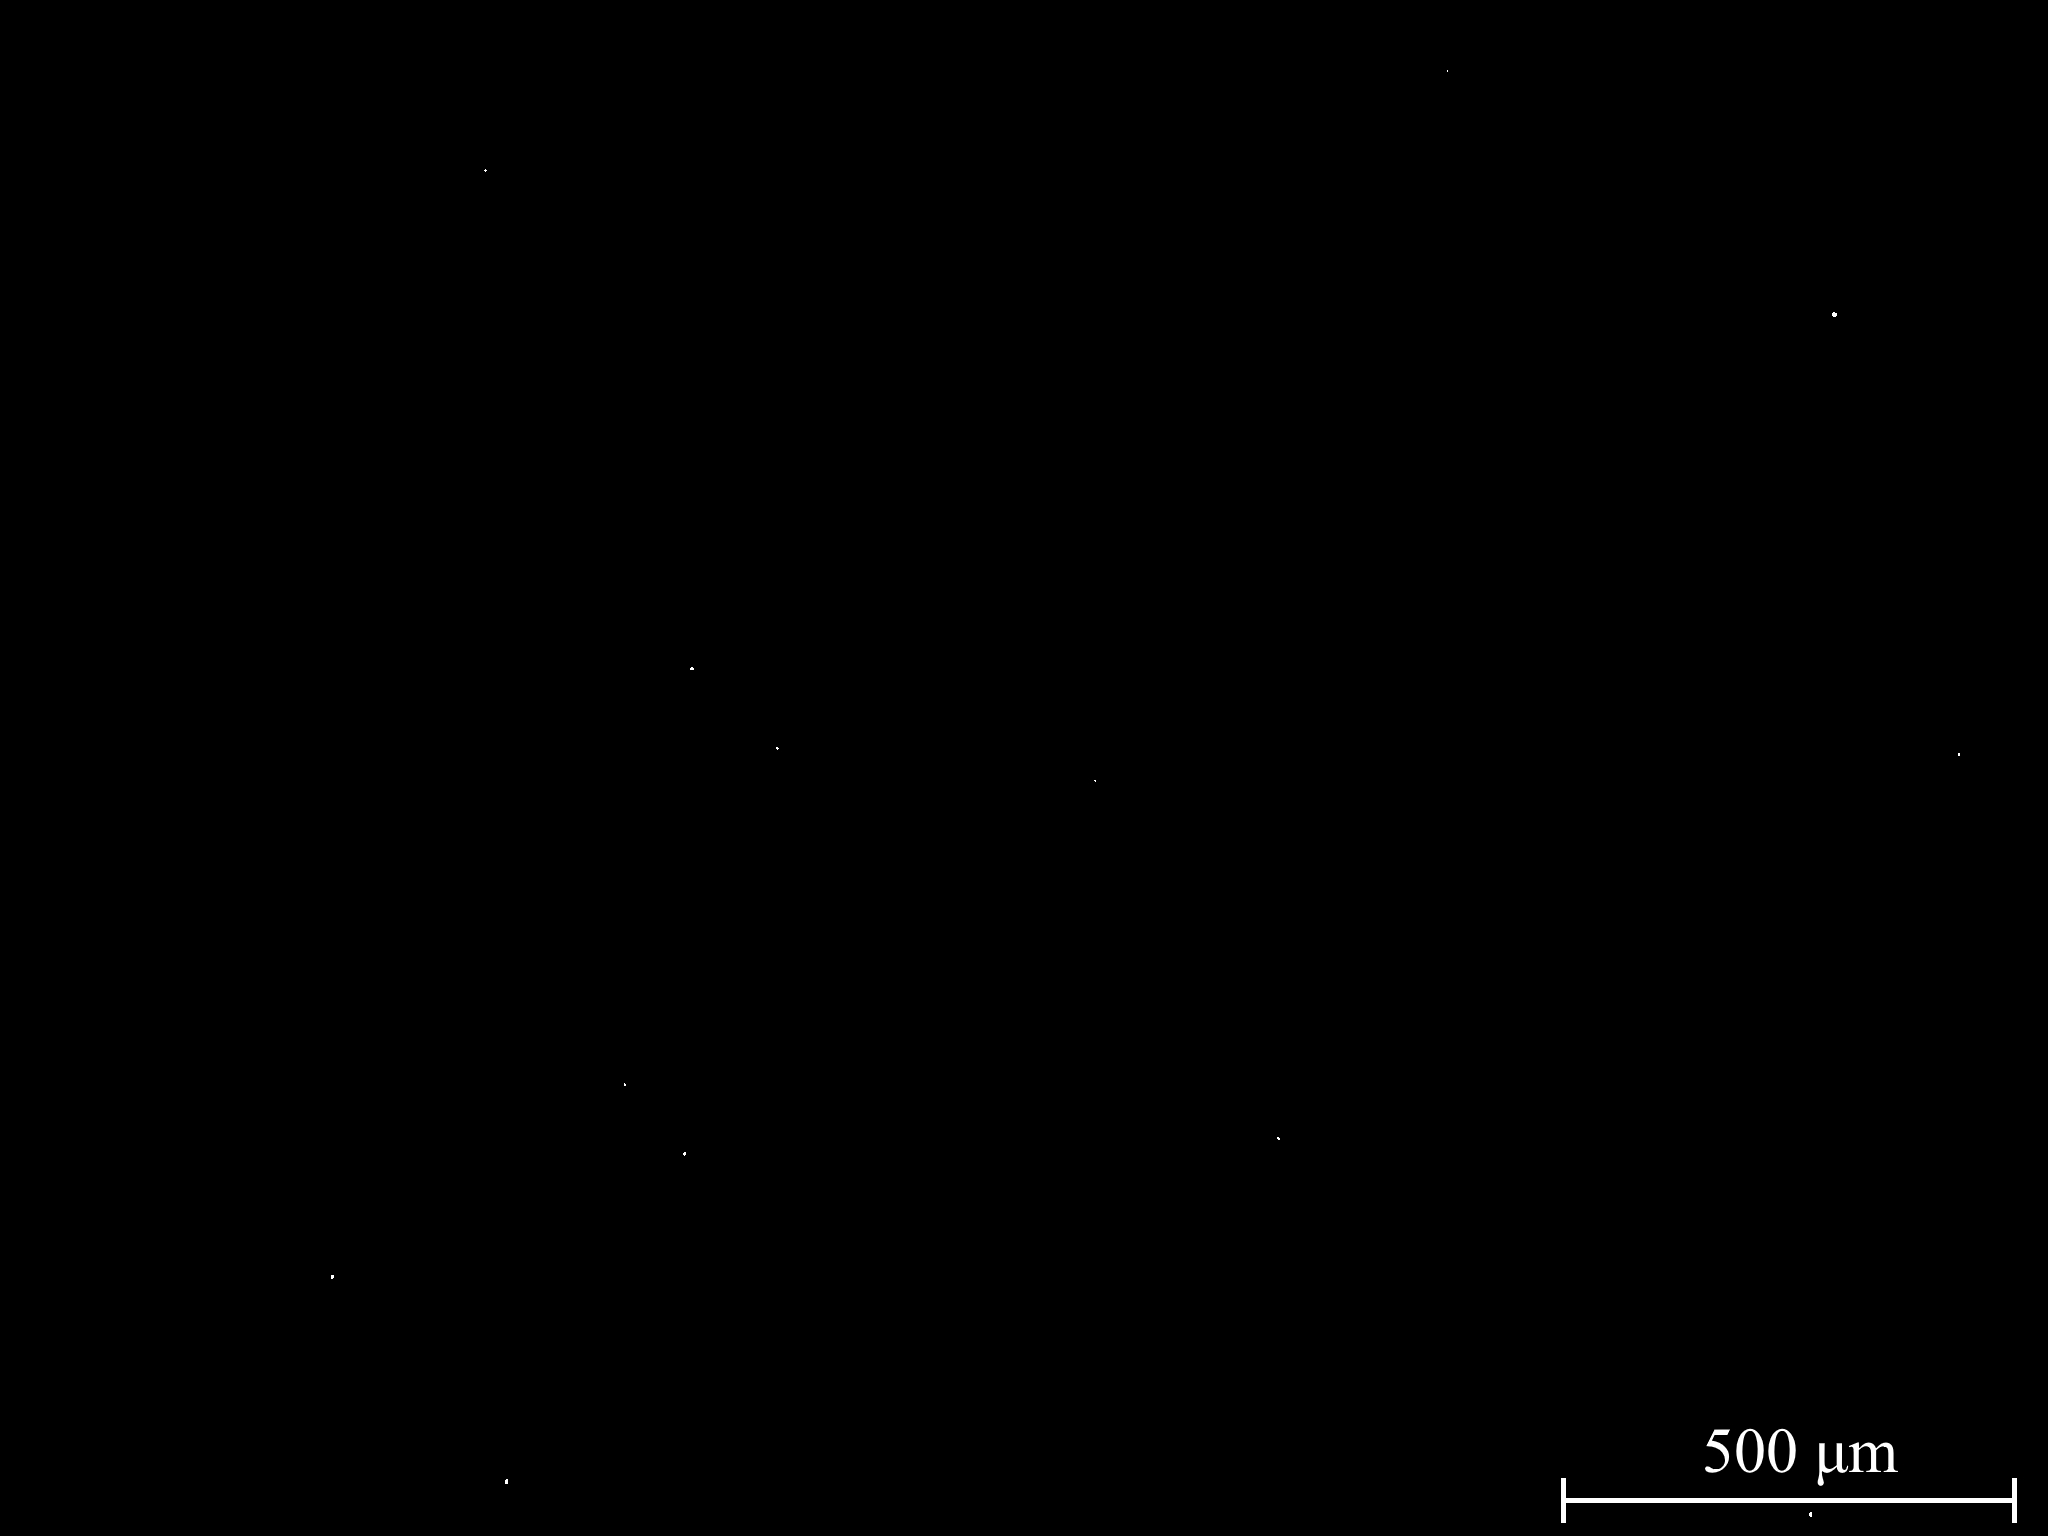
\includegraphics[width=0.8\linewidth]{subAb_om_df_n021.jpg}
    \caption[Dark field optical microscopy image of substrate A after a \ce{Br}:methanol etch.]{Dark field optical microscopy image of substrate A after a \ce{Br}:methanol etch taken near the centre of the substrate.\todo{Bedre bilde? Helt svart.}}\label{fig:subAb_om_df}
\end{figure}

\Ac{sem} shows the surface at a higher magnification and it reveals that there are much smaller particles distributed over the surface as well. Fig.~\ref{fig:subAb_sem_typical_centre} shows a typical image of an area near the centre of the substrate. Here the particle density is  \SI{\sim 2e+06}{\particle\centi\metre^{-2}}. The highest observed density of particles is counted near the upper edge to be \SI{3e+07}{\particle\centi\metre^{-2}}, see Fig.~\ref{fig:subAb_sem_typical_edge}.

\begin{figure}[htbp]
    \mySubfigure{0.49\textwidth}{subAb_sem_02b_m008.png}[fig:subAb_sem_typical_centre]
    \hfill
    \mySubfigure{0.49\textwidth}{subAb_sem_02a_m004.png}[fig:subAb_sem_typical_edge]
    \caption[\Ac{sem} images of typical areas on substrate A after a \ce{Br}:methanol etch.]{\Ac{sem} images of \subref{fig:subAb_sem_typical_centre} a typical area near the centre and \subref{fig:subAb_sem_typical_edge} an area with a high density of particles near the edge of substrate A after a \ce{Br}:methanol etch.\todo{Sett inn bilder uten kontrast-endring.}}\label{fig:subAb_sem_typical}
\end{figure}

%%=========================================
\subsection{Particles}
Four different types of particles are found on the surface of substrate A after a \ce{Br}:methanol etch, see Fig.~\ref{fig:subAb_sem_w_eds}.

\begin{figure}
    \centering
    \begin{subfigure}[t]{\textwidth}
        \caption{}\label{fig:subAb_silica}
          \begin{minipage}[t]{0.43\linewidth}
            \centering
            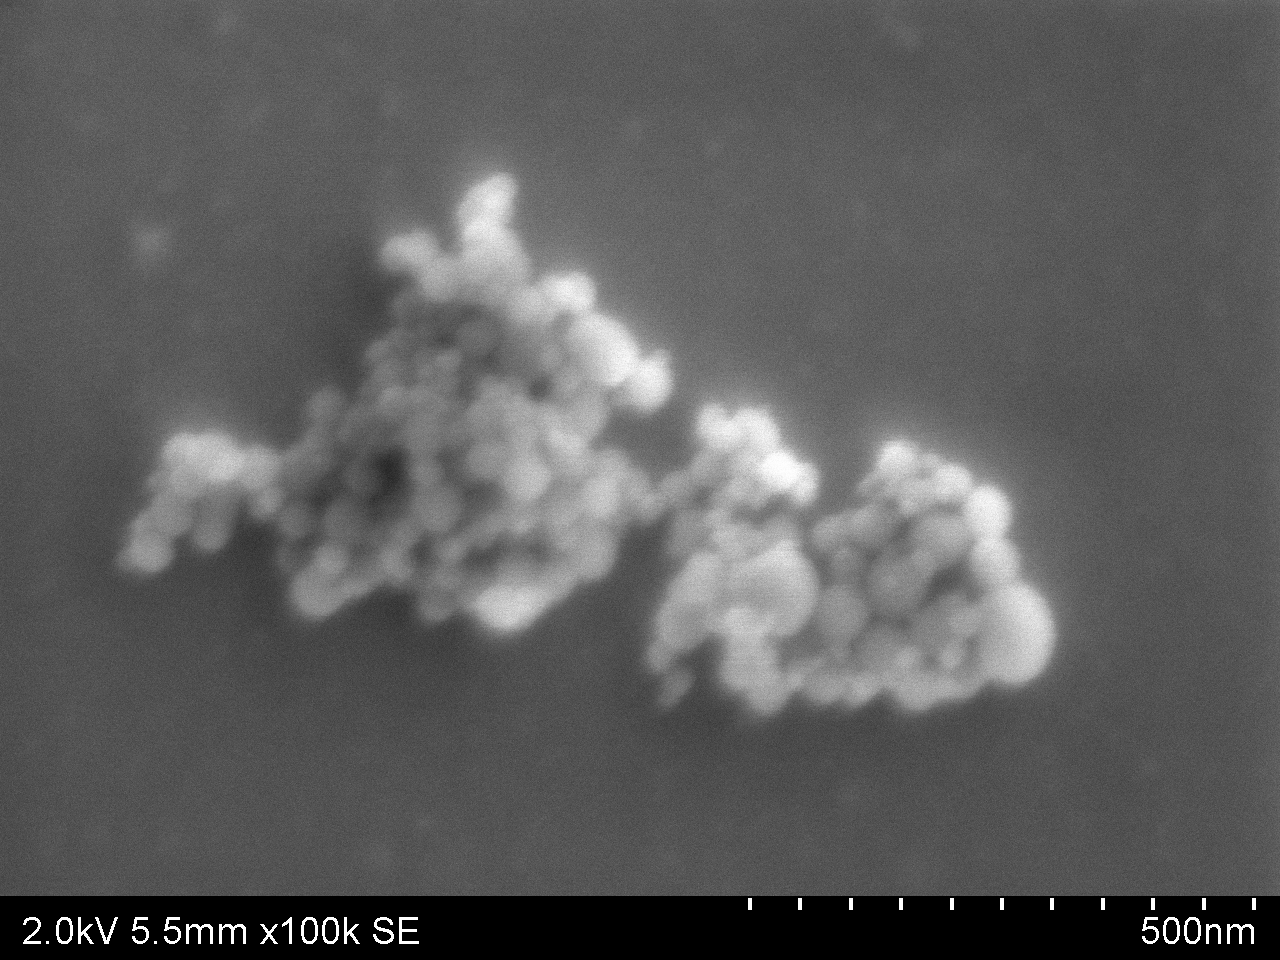
\includegraphics[width=\linewidth]{subAb_sem_03_m004.png}
          \end{minipage}
          \hfill
          \begin{minipage}[t]{0.43\linewidth}
            \centering
            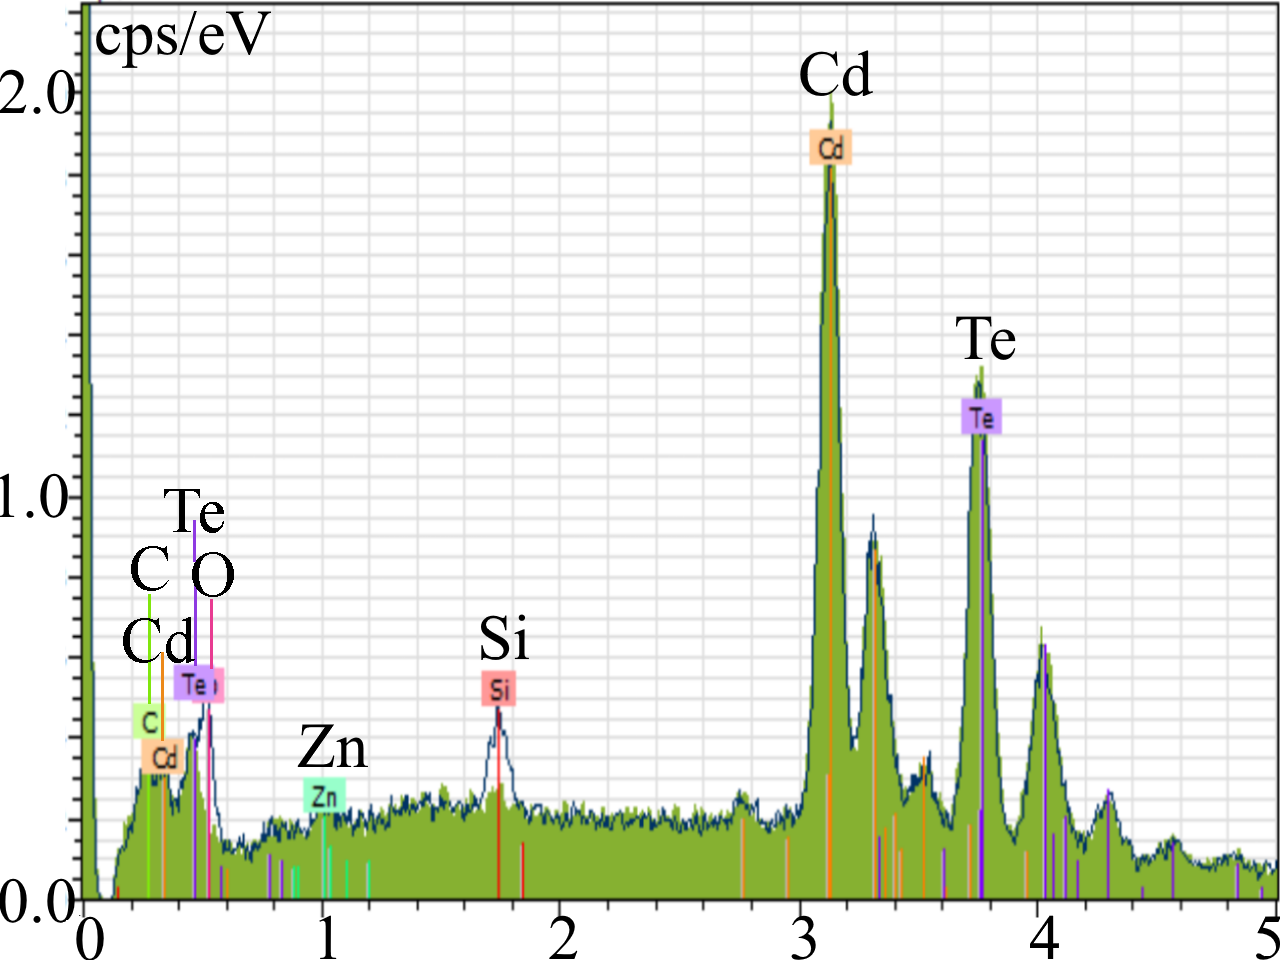
\includegraphics[width=\linewidth]{subAb_eds_03_m004.png}
          \end{minipage}
          \begin{minipage}[t]{0.11\linewidth}
            \centering
            \atomicTable[&][&][&]
          \end{minipage}
    \end{subfigure}
    \par\bigskip
    \begin{subfigure}[t]{\textwidth}
        \caption{}\label{fig:subAb_silica2}
          \begin{minipage}[t]{0.43\linewidth}
            \centering
            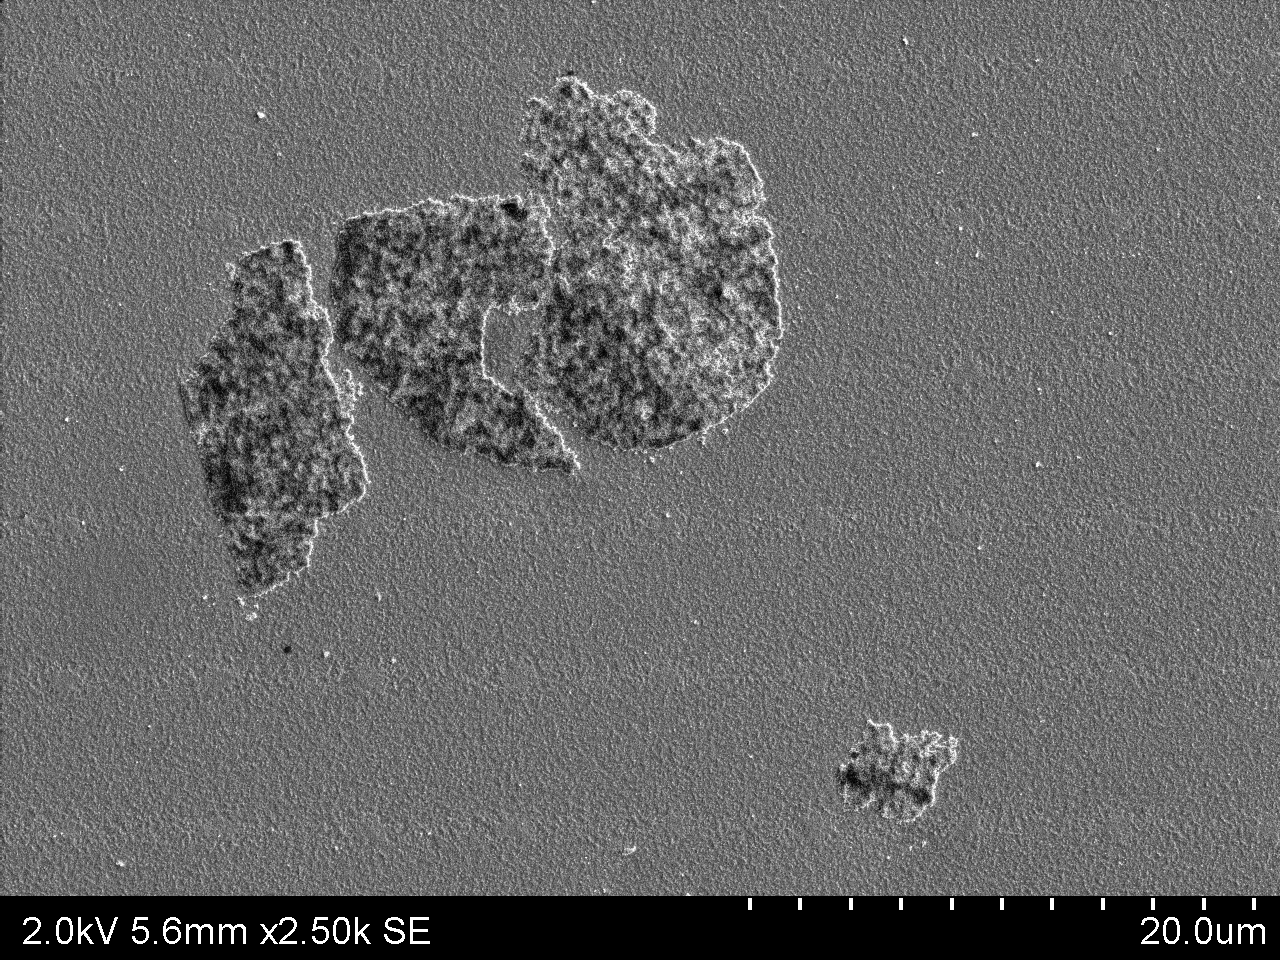
\includegraphics[width=\linewidth]{subAb_sem_03_m005.png}
          \end{minipage}
          \hfill
          \begin{minipage}[t]{0.43\linewidth}
            \centering
            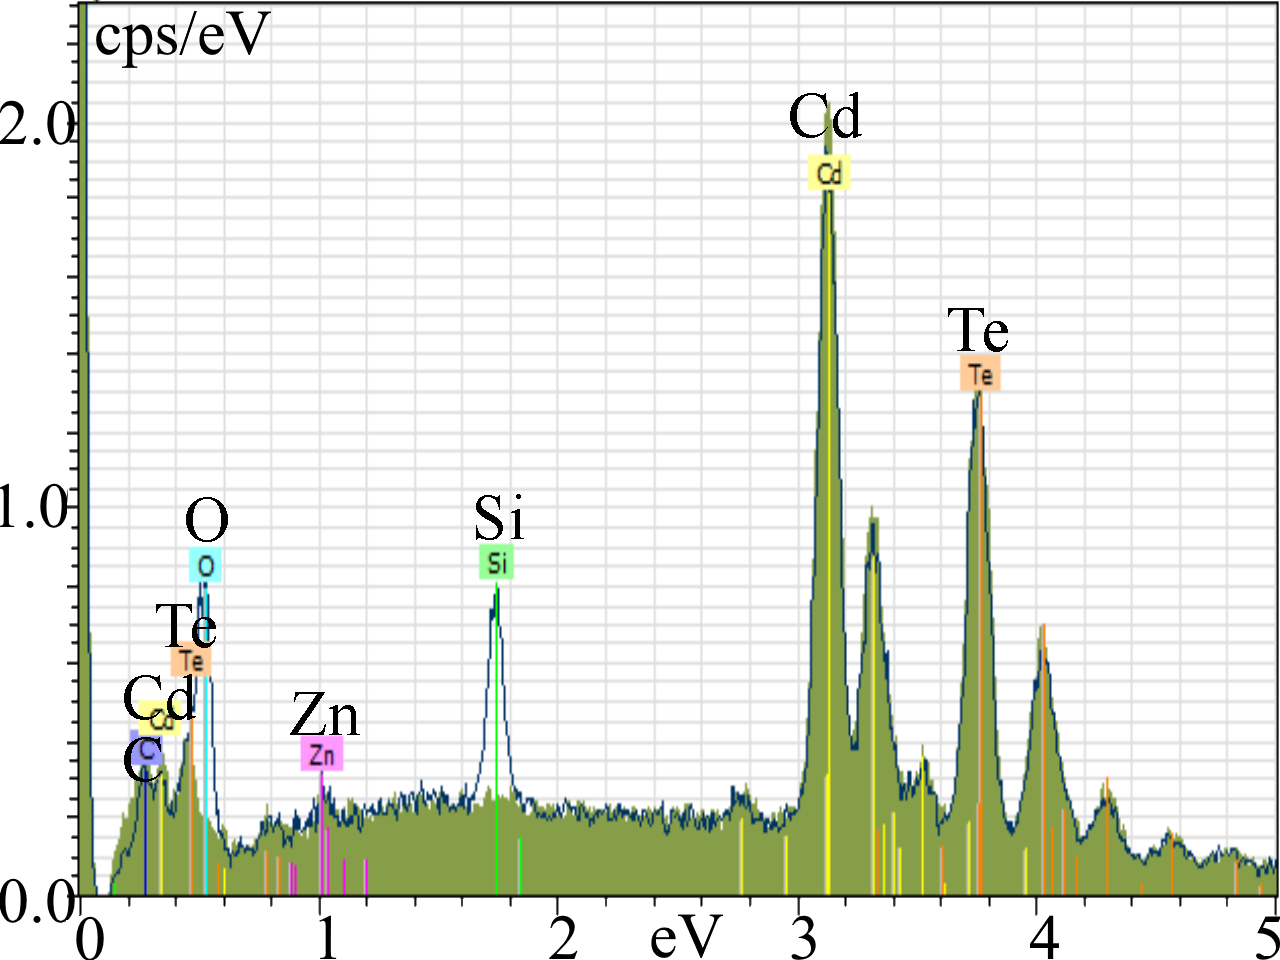
\includegraphics[width=\linewidth]{subAb_eds_03_m005.png}
          \end{minipage}
          \begin{minipage}[t]{0.11\linewidth}
            \centering
            \atomicTable[&][&][&]
          \end{minipage}
    \end{subfigure}
    \par\bigskip
    \begin{subfigure}[t]{\textwidth}
        \caption{}\label{fig:subAb_br-stain}
          \begin{minipage}[t]{0.43\linewidth}
            \centering
            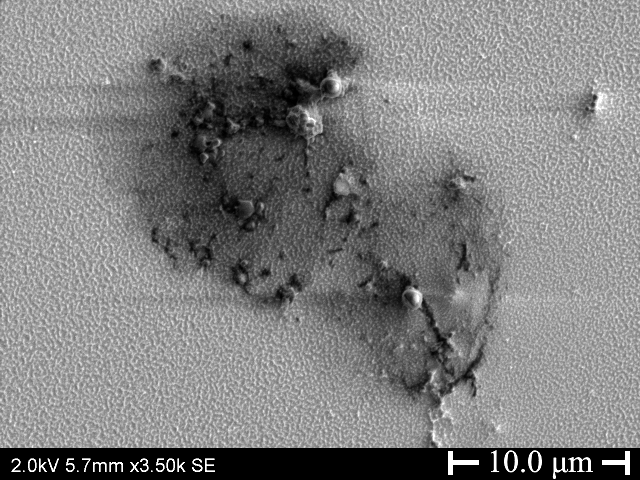
\includegraphics[width=\linewidth]{subAb_sem_03_m011.png}
          \end{minipage}
          \hfill
          \begin{minipage}[t]{0.43\linewidth}
            \centering
            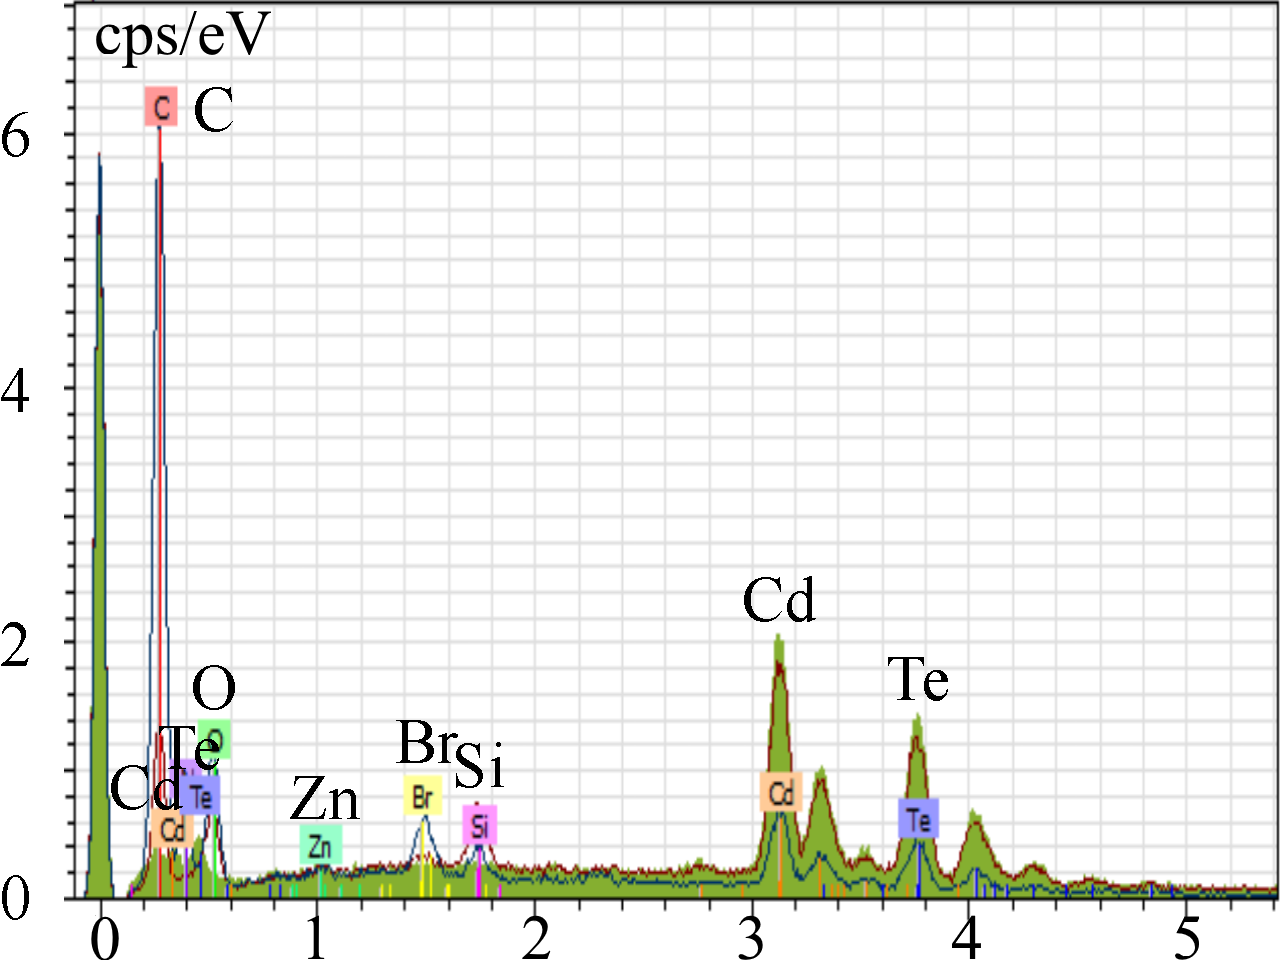
\includegraphics[width=\linewidth]{subAb_eds_03_m011.png}
          \end{minipage}
          \begin{minipage}[t]{0.11\linewidth}
            \centering
            \atomicTable[&][&][&]
          \end{minipage}
    \end{subfigure}
    \caption[\Ac{sem} images, \ac{eds} spectra, and \ac{eds} atomic compositions of three different types of particles and one type of stain found on substrate A after a \ce{Br}:methanol etch.]{High resolution \ac{sem} images of four different types of particles and one stain found on substrate A after a \ce{Br}:methanol etch and the corresponding \ac{eds} spectra and atomic compositions: \subref{fig:subAb_silica} Silica (\ce{SiO2}) polishing grit agglomeration; \subref{fig:subAb_silica2} silica (\ce{SiO2}) particles; \subref{fig:subAb_br-stain} stain consisting of bromine, carbon, and oxygen; and \subref{fig:subAb_br-particle} particle consisting of bromine, carbon, and oxygen. The blue line represents the \ac{eds} spectrum of the particle, while the filled green represents the \ac{eds} spectrum of the underlying substrate.}\label{fig:subAb_sem_w_eds}
\end{figure}
%
\begin{figure}[htbp]
\ContinuedFloat
    \centering
    \begin{subfigure}[t]{\textwidth}
        \caption{}\label{fig:subAb_br-particle}
          \begin{minipage}[t]{0.43\linewidth}
            \centering
            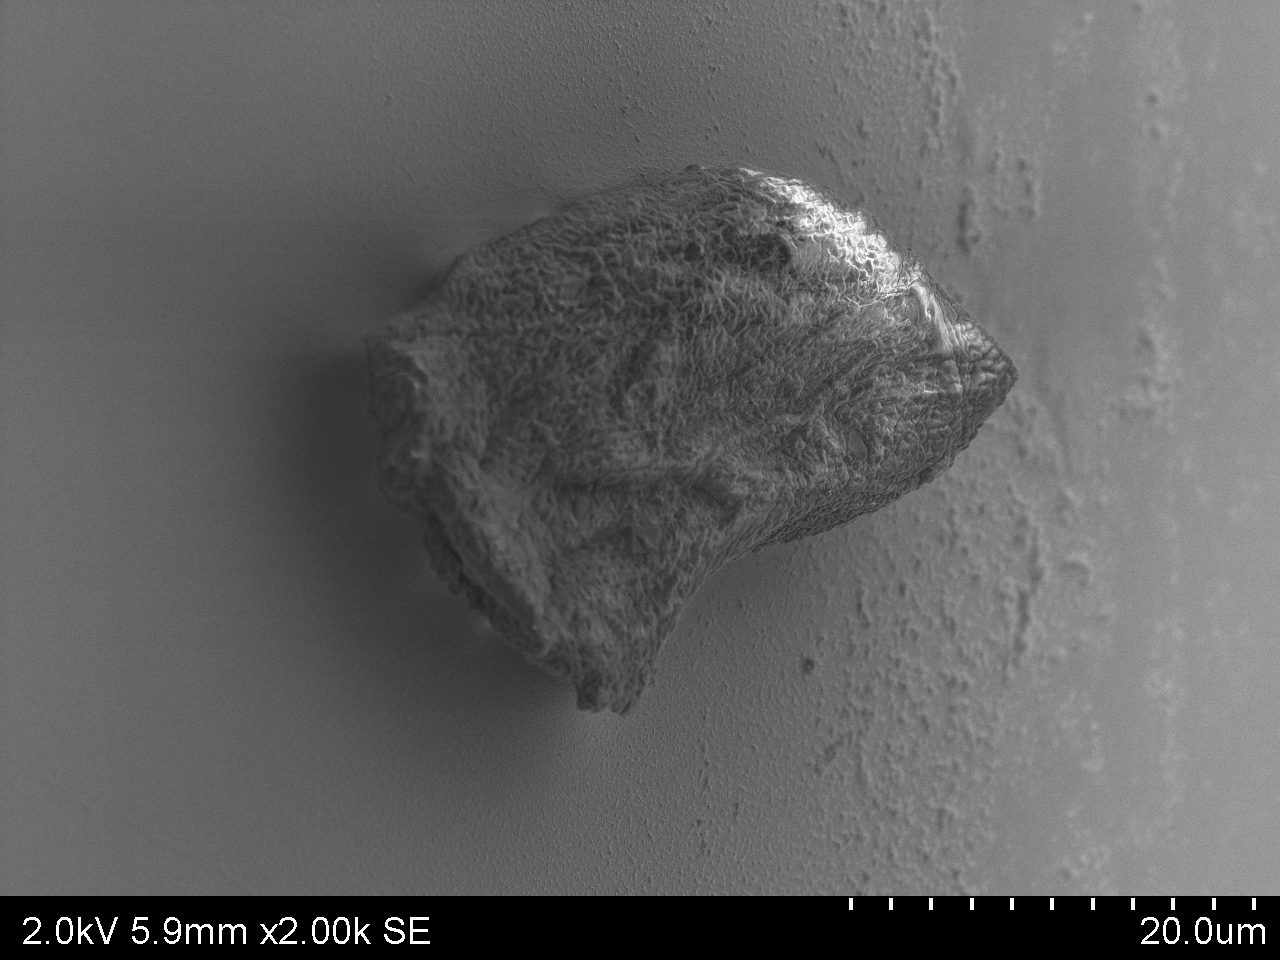
\includegraphics[width=\linewidth]{subAb_sem_03_m013.png}
          \end{minipage}
          \hfill
          \begin{minipage}[t]{0.43\linewidth}
            \centering
            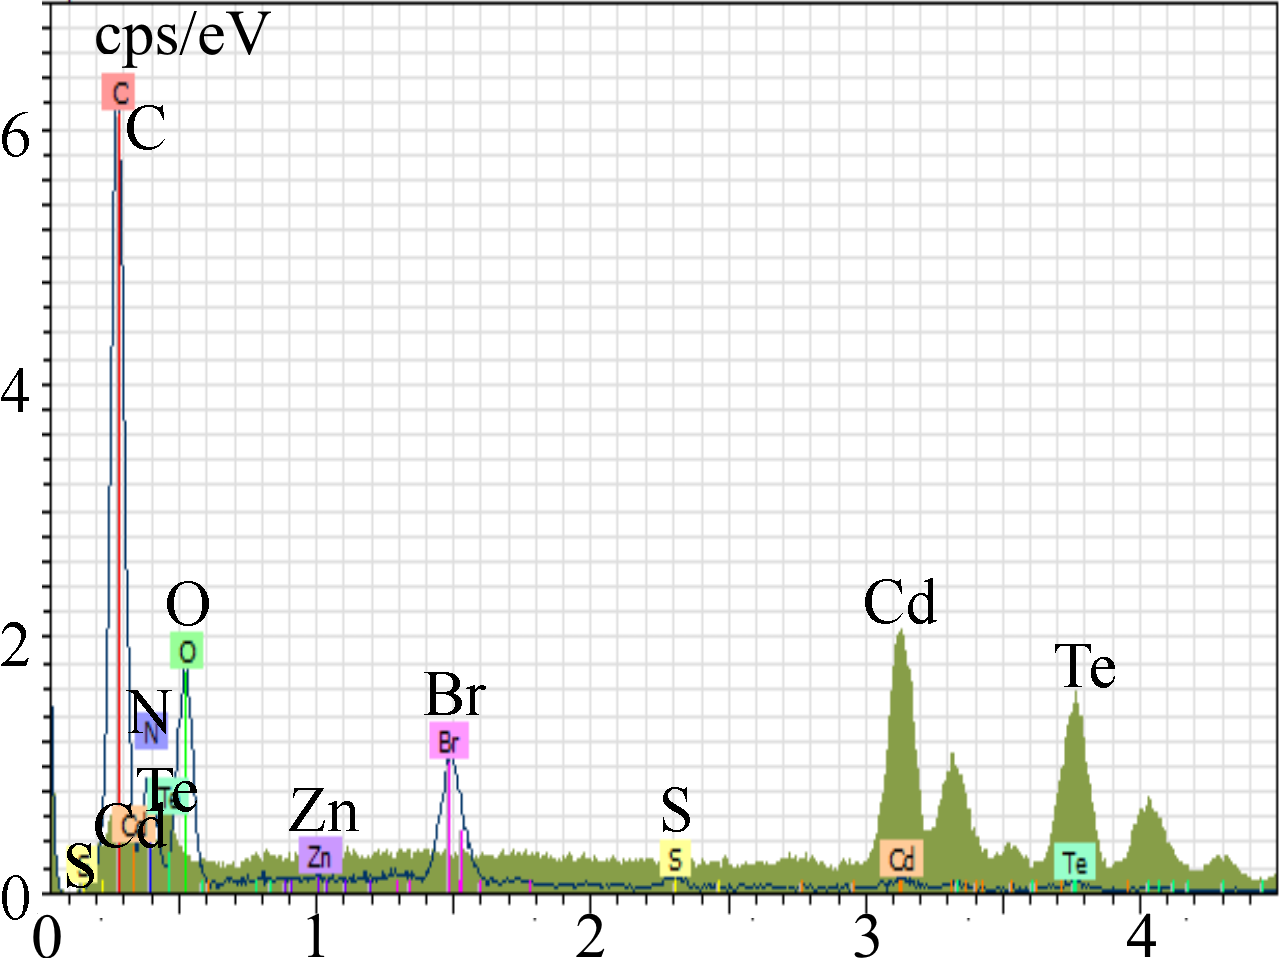
\includegraphics[width=\linewidth]{subAb_eds_03_m013.png}
          \end{minipage}
          \begin{minipage}[t]{0.11\linewidth}
            \centering
            \atomicTable[&][&][&]
          \end{minipage}
    \end{subfigure}
    \captionsetup{list=no}
    \caption{\emph{(continued)}}
\end{figure}

\subsubsection{Silica (\ce{SiO2}) polishing grit and flake}

As before the \ce{Br}:methanol etch, silica polishing grit is found on the surface of the substrate, see Fig.~\ref{fig:subAb_silica}. However, the grit density is higher and there are larger agglomerations of grit. The polishing grit may originate from the sides edges or bottom surface of the as-received substrate and have been distributed over the surface by the etch solution.

The silica polishing grit observed in \ac{sem} are found all over the surface. The particle density was found to be between \SI{2e+06}{\particle\centi\metre^{-2}} and \SI{3e+07}{\particle\centi\metre^{-2}}. The mean particle density was \SI{7e+06}{\particle\centi\metre^{-2}} with a standard deviation of \SI{7e+06}{\particle\centi\metre^{-2}}. A graphical representation of the particle density at different locations on substrate A can be seen in Fig.~\ref{fig:subAb_densityData}. There is a tendency of higher density towards the upper right and lower left corners.

\begin{figure}[htbp]
    \centering
    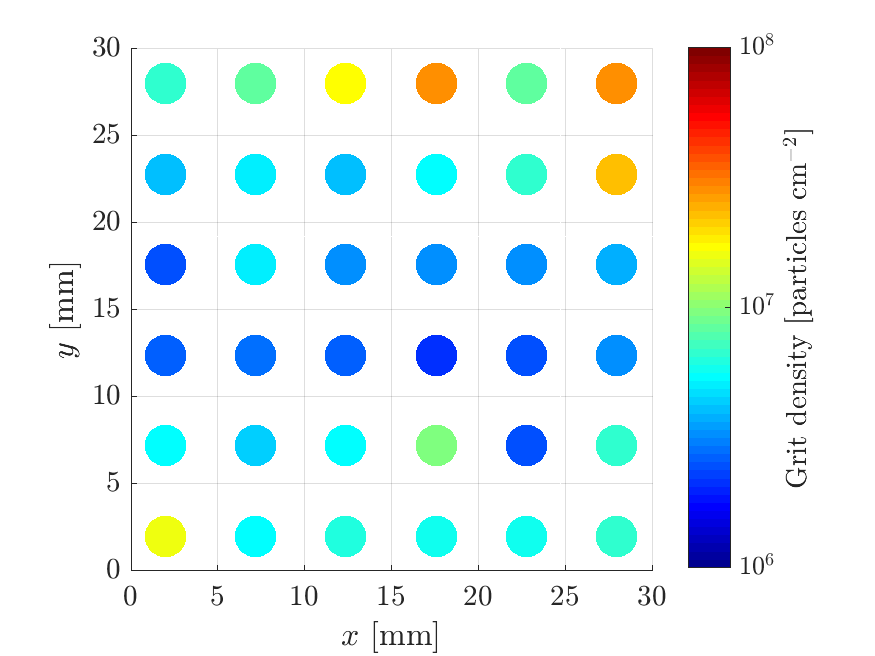
\includegraphics[width=0.8\linewidth]{subAb_densityData.png}
    \caption[Map of the polishing grit density on substrate A after a \ce{Br}:methanol etch.]{A map of the polishing grit density at 36 different locations on the $\SI{30}{\milli\metre}\times\SI{30}{\milli\metre}$ substrate A after a \ce{Br}:methanol etch. The polishing grit density was observed to vary between \SI{2e+06}{\particle\centi\metre^{-2}} and \SI{3e+07}{\particle\centi\metre^{-2}}.}
    \label{fig:subAb_densityData}
\end{figure}

Fig.~\ref{fig:subAb_silica2} shows four particles ranging from \SI{4}{\micro\metre} to \SI{15}{\micro\metre} in size. These particles consists of \ce{SiO2}. When looking at the particles at higher magnification, see Fig.~\ref{fig:subAb_silica2_magnified}, it appears that they are made up of smaller, circular particles with a diameter of \SIrange{50}{100}{\nano\metre}. Clearly, silica polishing grit have accumulated to a larger structure. These structures are mainly observed near the edges of the substrate.

\begin{figure}
    \centering
    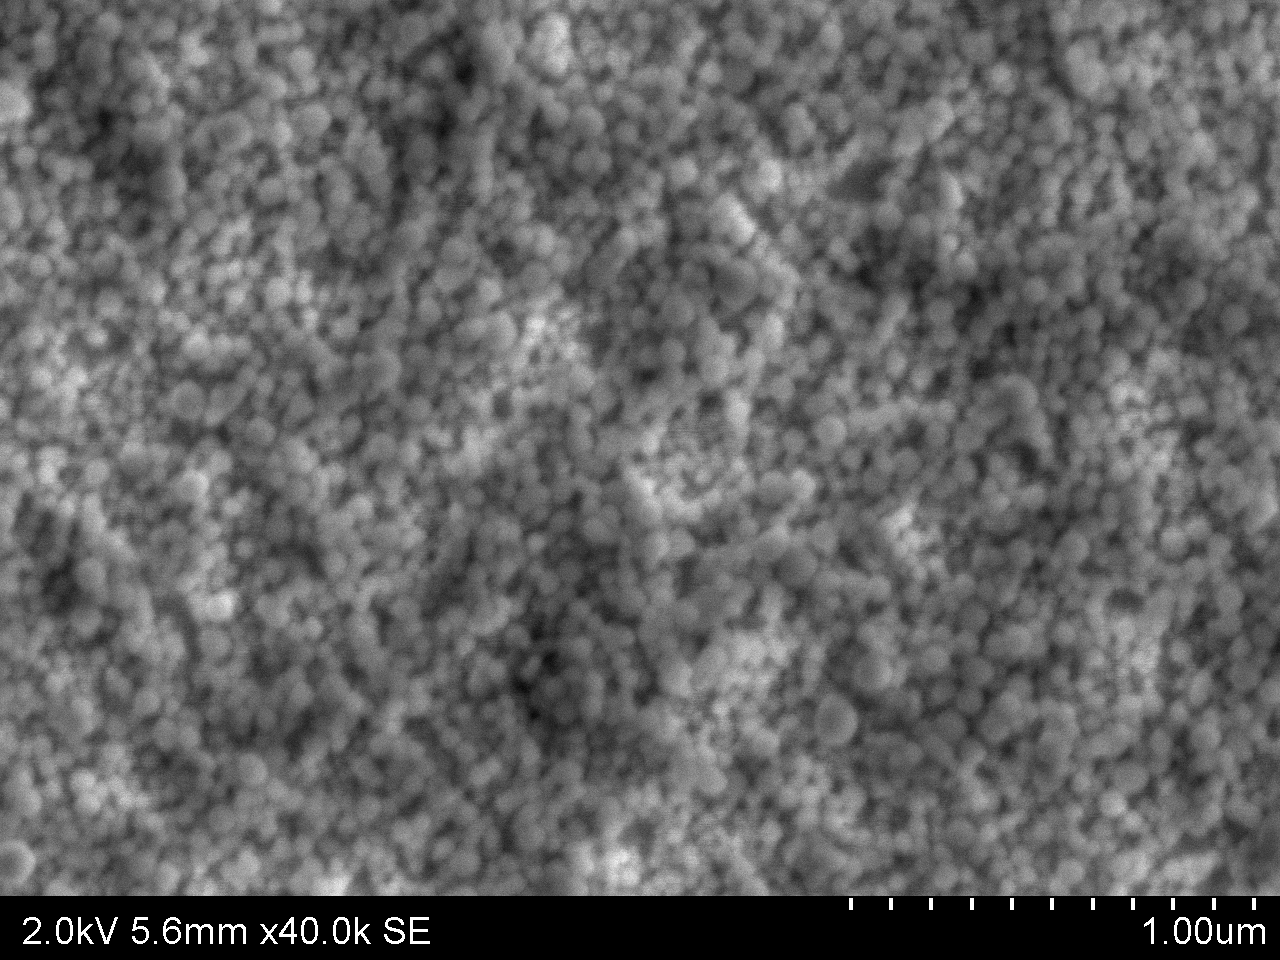
\includegraphics[width=0.8\linewidth]{subAb_sem_03_m006.png}
    \caption[\Ac{sem} image of silica flake.]{\Ac{sem} image of flake consisting of silica (\ce{SiO2}).}\label{fig:subAb_silica2_magnified}
\end{figure}

\subsubsection{Stain and particle based on bromine, oxygen and carbon}

Fig.~\ref{fig:subAb_br-stain} shows a stain that consists of bromine, carbon, and oxygen. This type of stain is observed mainly near the edges of substrate A. The stains are typically \SI{\sim10}{\micro\metre} long. Another type of particle showing the same composition in the \ac{eds} spectrum as the stain is also found around the edges of the substrate, see Fig.~\ref{fig:subAb_br-particle}. This particle is typically \SIrange{20}{30}{\micro\metre} long.

%%=========================================
%\section{AFM Study of Etched Substrate A}
\subsection{Surface Roughness}

The \ce{Br}:methanol etched substrate A was characterised for surface topography by \ac{afm}. Images of $\SI{5}{\micro\metre}\times\SI{5}{\micro\metre}$ areas were taken at three different locations on the substrate surface: near the centre, near the upper edge, and near the upper left corner, as seen in Fig.~\ref{fig:subAb_afm}. The \ac{rms} roughness was calculated using Eq.~\ref{eq:rmsroughness} to be \SI{0.51}{\nano\metre}, \SI{1.3}{\nano\metre}, and \SI{1.9}{\nano\metre} respectively. This is an increase in roughness by 2 near the centre, 4 near the edge, and 6 near the corner. The centre has a flat surface with particles with sizes between \SIrange{10}{50}{\nano\metre}, while the edge and corner have a pebbled surface, which makes it hard to see the presence of particles, as seen in Fig.~\ref{fig:subAb_afm_edge}--\oldsubref{fig:subAb_afm_corner}. The surface scratches from before the etch has disappeared, but the presence of polishing particles have increased the roughness of the surface.

\begin{figure}[htbp]
    \centering
    \begin{subfigure}[b]{0.032\linewidth}
        \label{fig:subAb_afm_scale}\captionsetup{list=no}
        
\includegraphics[width=\linewidth]{subAb_afm_scale.png}
    \end{subfigure}
    \hfill
    \mySubfigure{0.3\linewidth}{subAb_afm_centre.png}[fig:subAb_afm_centre] %\SI{0.85}{\nano\metre}
    \hfill
    \mySubfigure{0.3\linewidth}{subAb_afm_upperedge.png}[fig:subAb_afm_edge] %\SI{0.77}{\nano\metre}}
    \hfill
    \mySubfigure{0.3\linewidth}{subAb_afm_upperleftcorner.png}[fig:subAb_afm_corner]%\SI{1,04}{\nano\metre}
    \caption[\Ac{afm} of substrate A after a \ce{Br}:methanol etch.]{\Ac{afm} measurements of substrate A after a \ce{Br}:methanol etch. Images of $\SI{5}{\micro\metre}\times\SI{5}{\micro\metre}$ areas are taken at three different locations on the substrate surface: \subref{fig:subAb_afm_centre} near the centre, \ac{rms} roughness \SI{0.51}{\nano\metre}; \subref{fig:subAb_afm_edge} near the upper edge, \ac{rms} roughness \SI{1.3}{\nano\metre}; and \subref{fig:subAb_afm_corner} near the upper left corner, \ac{rms} roughness \SI{1.9}{\nano\metre}.}\label{fig:subAb_afm}
\end{figure} % AFM, substrate A, with surface pre-growth preparation.

%%=========================================
\subsection{Impurity Analysis}
\Ac{eds} was used to get a quantitative analysis of the chemical composition of substrate A after a \ce{Br}:methanol etch. The results can be seen in Table~\ref{tab:subAb_eds_analysis}. The following elements were identified: \ce{Te}, \ce{Cd}, \ce{Zn}, \ce{Al}, \ce{Si}, \ce{C}, and \ce{O}. The relative concentrations of \ce{Cd}, \ce{Zn}, and \ce{Te} had an error of less than one percentage point from the expected value of \SI{48}{\atomic\percent} cadmium, \SI{2}{\atomic\percent} zinc and \SI{50}{\atomic\percent} tellurium. The atomic concentration of alumina is two times as large near the corner as near the edge and centre. This was the case even before etch. In addition, the atomic concentration of oxygen is not high enough to be contributing to \ce{Al2O3} and \ce{SiO2} for all the detected aluminium and silicon, which may indicate that the substrate has inherent aluminium or silicon contamination as well as polishing grit.

\begin{table}[htbp]
    \centering
    \caption[\Ac{eds} impurity analysis of substrate A after a \ce{Br}:methanol etch.]{Results of the \ac{eds} impurity analysis at three different locations on the $30\times30$ \SI{}{\milli\metre^2} (111)B \ac{czt} substrate A after a \ce{Br}:methanol etch (atomic concentration \%). The X-ray signal is acquired from $\SI{1270}{\micro\metre}\times\SI{890}{\micro\metre}$ areas near the centre, upper edge, and upper left corner.}\label{tab:subAb_eds_analysis}
   \begin{tabu} to 1.0\textwidth { X[1.85, r] X[1.125,c] X[1.125,c] X[1.125,c] X[1.125,c] X[1.125,c] X[1.125,c] X[1.125,c] } % X[1,c] X[1,c]
        \hline
            & \textbf{\ce{Te}} (at.\%) & \textbf{\ce{Cd}} (at.\%) & \textbf{\ce{Zn}} (at.\%) & \textbf{\ce{Al} } (at.\%) & \textbf{\ce{Si}} (at.\%) & \textbf{\ce{C}} (at.\%) & \textbf{\ce{O}} (at.\%) \\ % \textbf{$X$} (\SI{}{\milli\metre}) &  \textbf{$Y$} (\SI{}{\milli\metre})
        \hline
        Near centre & \SI{45.42}{} & \SI{44.95}{} & \SI{1.84}{} & \SI{0.22}{} & \SI{0.54}{} & \SI{6.05}{} & \SI{0.97}{} \\ % \SI{15.0}{} & \SI{15.0}{}
        Near edge & \SI{45.41}{} & \SI{45.08}{} & \SI{1.72}{} & \SI{0.25}{} & \SI{0.60}{} & \SI{6.01}{} & \SI{0.95}{} \\ % \SI{15.0}{} & \SI{29.0}{} 
        Near corner & \SI{45.18}{} & \SI{44.79}{} & \SI{1.70}{} & \SI{0.56}{} & \SI{0.63}{} & \SI{6.45}{} & \SI{0.70}{} \\ % \SI{1.0}{}  & \SI{29.0}{}
        \hline
    \end{tabu}
\end{table}
%%=========================================

